\hypertarget{o-que-uxe9-um-compilador}{%
\section{O que é um Compilador?}\label{o-que-uxe9-um-compilador}}

\begin{frame}{Defini\c{c}\~{a}o}
\protect\hypertarget{definiuxe7uxe3o}{}
\begin{itemize}

\item
  Um compilador \textbf{traduz} um programa de uma linguagem de origem
  para uma de destino
\item
  A linguagem de origem é projetada para ser \textbf{compreensível por
  humanos}
\end{itemize}
\end{frame}

\begin{frame}{Defini\c{c}\~{a}o}
\protect\hypertarget{definiuxe7uxe3o-1}{}
\begin{itemize}

\item
  A linguagem de destino é projetada para \textbf{execu\c{c}\~{a}o eficiente por
  hardware}
\item
  A tradu\c{c}\~{a}o é desafiadora quando as linguagens s\~{a}o muito diferentes
\end{itemize}
\end{frame}

\begin{frame}{Defini\c{c}\~{a}o}
\protect\hypertarget{definiuxe7uxe3o-2}{}
\begin{itemize}

\item
  Compiladores s\~{a}o sistemas complexos que exigem técnicas sofisticadas
\end{itemize}
\end{frame}

\begin{frame}{Exemplos de Compila\~{c}\~{a}o}
\protect\hypertarget{exemplos-de-compilauxe7uxe3o}{}
\begin{itemize}

\item
  C/C++ → código assembly x86-64
\item
  Java → bytecode JVM (\emph{just-in-time}: JVM → código nativo)
\end{itemize}
\end{frame}

\begin{frame}{Exemplos de Compila\~{c}\~{a}o}
\protect\hypertarget{exemplos-de-compilauxe7uxe3o-1}{}
\begin{itemize}

\item
  Haskell → código assembly via GHC
\item
  TypeScript → JavaScript
\item
  LLVM IR → código de máquina para diversas arquiteturas
\end{itemize}
\end{frame}

\begin{frame}{Compiladores vs.~Interpretadores}
\protect\hypertarget{compiladores-vs.-interpretadores}{}
\begin{longtable}[]{@{}lll@{}}
\toprule\noalign{}
& Compilador & Interpretador \\
\midrule\noalign{}
\endhead
Execu\c{c}\~{a}o & Traduz antes de executar & Executa diretamente \\
Desempenho & \textasciitilde10× mais rápido & Mais lento \\
\bottomrule\noalign{}
\end{longtable}
\end{frame}

\begin{frame}{Compiladores vs.~Interpretadores}
\protect\hypertarget{compiladores-vs.-interpretadores-1}{}
\begin{longtable}[]{@{}lll@{}}
\toprule\noalign{}
& Compilador & Interpretador \\
\midrule\noalign{}
\endhead
Energia & Menos consumo & Mais consumo \\
Tempo de compila\~{c}\~{a}o & Pode ser alto & Nenhum \\
\bottomrule\noalign{}
\end{longtable}
\end{frame}

\begin{frame}{Compiladores vs.~Interpretadores}
\protect\hypertarget{compiladores-vs.-interpretadores-2}{}
\begin{itemize}

\item
  Compilar faz sentido para programas executados \textbf{muitas vezes}
\item
  Para execu\c{c}\~{a}o única, interpretar pode ser mais conveniente
\end{itemize}
\end{frame}

\begin{frame}{Por que Compiladores S\~{a}o Difíceis?}
\protect\hypertarget{por-que-compiladores-suxe3o-difuxedceis}{}
\begin{itemize}

\item
  Código-fonte: legível, estruturado, redundante, favorece análise
\item
  Código-alvo: compacto, eficiente, pouco legível, descarta estrutura de
  alto nível
\end{itemize}
\end{frame}

\begin{frame}{Por que Compiladores S\~{a}o Difíceis?}
\protect\hypertarget{por-que-compiladores-suxe3o-difuxedceis-1}{}
\begin{itemize}

\item
  A diferen\c{c}a entre as duas representa\c{c}\~{o}es é enorme
\item
  Mais importante que desempenho é a \textbf{corre\c{c}\~{a}o} do compilador
\item
  Erros introduzidos pelo compilador s\~{a}o extremamente difíceis de
  depurar
\end{itemize}
\end{frame}

\begin{frame}{Corre\c{c}\~{a}o de Compiladores}
\protect\hypertarget{correuxe7uxe3o-de-compiladores}{}
\begin{itemize}

\item
  É possível definir matematicamente o que significa um compilador estar
  correto
\item
  Requer sem\^{a}ntica formal para linguagem de origem \textbf{e} de destino
\end{itemize}
\end{frame}

\begin{frame}{Corre\c{c}\~{a}o de Compiladores}
\protect\hypertarget{correuxe7uxe3o-de-compiladores-1}{}
\begin{itemize}

\item
  Vários compiladores foram desenvolvidos com \textbf{provas de
  corre\c{c}\~{a}o}
\item
  Exemplo: CompCert --- compilador C com prova formal verificada por
  computador
\item
  Nossa abordagem: especificar cada fase com precis\~{a}o
\end{itemize}
\end{frame}

\hypertarget{fases-de-um-compilador}{%
\section{Fases de um Compilador}\label{fases-de-um-compilador}}

\begin{frame}{Vis\~{a}o Geral do Pipeline}
\protect\hypertarget{visuxe3o-geral-do-pipeline}{}
\begin{enumerate}

\item
  \textbf{Análise léxica} --- caracteres → tokens
\item
  \textbf{Análise sintática} --- tokens → árvore sintática
\item
  \textbf{Análise sem\^{a}ntica} --- verifica\c{c}\~{a}o de tipos e de contexto
\end{enumerate}
\end{frame}

\begin{frame}{Vis\~{a}o Geral do Pipeline}
\protect\hypertarget{visuxe3o-geral-do-pipeline-1}{}
\begin{enumerate}
\setcounter{enumi}{3}

\item
  \textbf{Gera\c{c}\~{a}o de código intermediário} --- árvore → representa\c{c}\~{a}o
  intermediária
\item
  \textbf{Otimiza\c{c}\~{a}o} --- melhora o código intermediário
\item
  \textbf{Gera\c{c}\~{a}o de código} --- representa\c{c}\~{a}o intermediária →
  código-alvo
\end{enumerate}
\end{frame}

\begin{frame}{A Ideia Central: Dividir para Conquistar}
\protect\hypertarget{a-ideia-central-dividir-para-conquistar}{}
\begin{itemize}

\item
  Em vez de traduzir diretamente do código-fonte para código de máquina
\item
  Definimos uma sequ\^{e}ncia de \textbf{fases} e \textbf{representa\c{c}\~{o}es
  intermediárias}
\end{itemize}
\end{frame}

\begin{frame}{A Ideia Central: Dividir para Conquistar}
\protect\hypertarget{a-ideia-central-dividir-para-conquistar-1}{}
\begin{itemize}

\item
  Cada fase transforma o programa para uma representa\c{c}\~{a}o mais próxima do
  destino
\item
  Cada representa\c{c}\~{a}o intermediária é projetada para a conveni\^{e}ncia da
  fase atual
\end{itemize}
\end{frame}

\begin{frame}[fragile]{Programa de Exemplo}
\protect\hypertarget{programa-de-exemplo}{}
\begin{lstlisting}
if (val >= 0) pos = val
\end{lstlisting}

\begin{itemize}

\item
  Vamos acompanhar essa instru\c{c}\~{a}o pelas fases do compilador
\item
  Come\c{c}amos com uma sequ\^{e}ncia de bytes/caracteres
\item
  Terminamos com instru\c{c}\~{o}es de máquina
\end{itemize}
\end{frame}

\begin{frame}[fragile]{Análise Léxica}
\protect\hypertarget{anuxe1lise-luxe9xica}{}
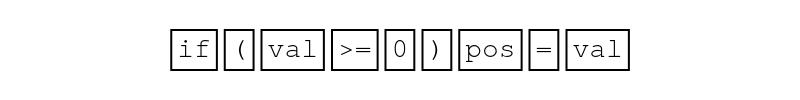
\includegraphics[width=0.7\textwidth,height=\textheight]{chapter01/imgs/lexical.png}

\begin{itemize}

\item
  Divide o texto em \textbf{tokens} (as ``palavras'' do programa)
\item
  Descarta espa\c{c}os em branco e comentários
\item
  Exemplo: \texttt{if}, \texttt{(},
  \texttt{val}, \texttt{>=},
  \texttt{0}, \texttt{)},
  \texttt{pos}, \texttt{=},
  \texttt{val}
\item
  Detecta erros léxicos: caracteres inválidos, identificadores
  malformados
\end{itemize}
\end{frame}

\begin{frame}{Análise Sintática}
\protect\hypertarget{anuxe1lise-sintuxe1tica}{}
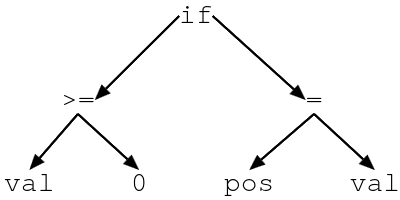
\includegraphics[width=0.4\textwidth,height=\textheight]{chapter01/imgs/syntax-tree.png}

\begin{itemize}

\item
  Verifica se os tokens formam uma sequ\^{e}ncia sintaticamente válida
\item
  Produz uma \textbf{Árvore Sintática Abstrata (AST)}
\end{itemize}
\end{frame}

\begin{frame}{Análise Sintática}
\protect\hypertarget{anuxe1lise-sintuxe1tica-1}{}
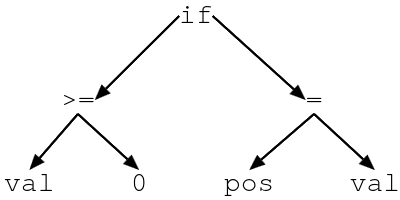
\includegraphics[width=0.4\textwidth,height=\textheight]{chapter01/imgs/syntax-tree.png}

\begin{itemize}

\item
  Captura a estrutura hierárquica do programa
\item
  Descarta elementos puramente sintáticos (como par\^{e}nteses)
\end{itemize}
\end{frame}

\begin{frame}{Análise Sem\^{a}ntica}
\protect\hypertarget{anuxe1lise-semuxe2ntica}{}
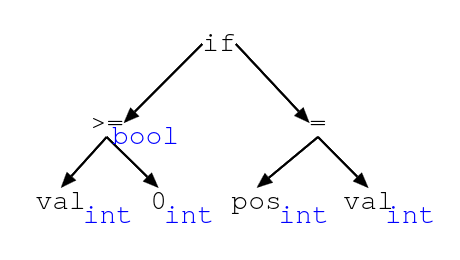
\includegraphics[width=0.4\textwidth,height=\textheight]{chapter01/imgs/annotated-tree.png}

\begin{itemize}

\item
  Completa a tarefa de verificar se o código representa um programa
  válido
\item
  Realiza \textbf{verifica\c{c}\~{a}o de tipos} e verifica\c{c}\~{o}es de contexto
\end{itemize}
\end{frame}

\begin{frame}{Análise Sem\^{a}ntica}
\protect\hypertarget{anuxe1lise-semuxe2ntica-1}{}
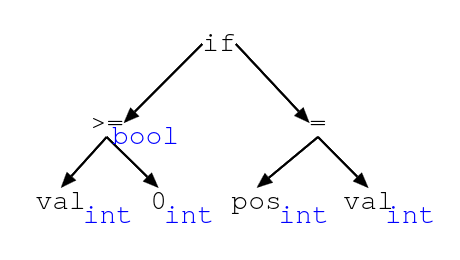
\includegraphics[width=0.4\textwidth,height=\textheight]{chapter01/imgs/annotated-tree.png}

\begin{itemize}

\item
  Coleta informa\c{c}\~{o}es adicionais sobre o programa
\item
  Enriquece a AST com \textbf{anota\c{c}\~{o}es} (tipos, refer\^{e}ncias a
  declara\c{c}\~{o}es)
\end{itemize}
\end{frame}

\begin{frame}{Gera\c{c}\~{a}o de Código Intermediário}
\protect\hypertarget{gerauxe7uxe3o-de-cuxf3digo-intermediuxe1rio}{}
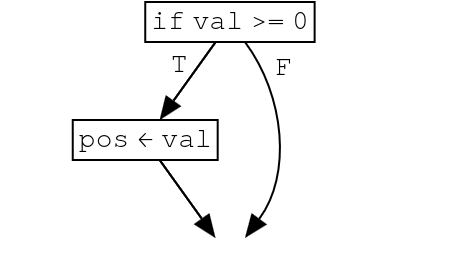
\includegraphics[width=0.4\textwidth,height=\textheight]{chapter01/imgs/cfg.png}

\begin{itemize}

\item
  Produz uma \textbf{Representa\c{c}\~{a}o Intermediária (RI)}
\item
  Exemplo: grafo de fluxo de controle
\end{itemize}
\end{frame}

\begin{frame}[fragile]{Sele\c{c}\~{a}o de Instru\c{c}\~{o}es}
\protect\hypertarget{seleuxe7uxe3o-de-instruuxe7uxf5es}{}
\begin{lstlisting}
     cmp val, 0       -- compara val com 0
     jl L1            -- salta se menor
     mov pos, val     -- pos = val
L1:
\end{lstlisting}

\begin{itemize}

\item
  Traduz a RI para instru\c{c}\~{o}es assembly abstrato
\item
  Variáveis ainda s\~{a}o tratadas como registradores virtuais
\end{itemize}
\end{frame}

\begin{frame}[fragile]{Aloca\c{c}\~{a}o de Registradores e Otimiza\c{c}\~{a}o}
\protect\hypertarget{alocauxe7uxe3o-de-registradores-e-otimizauxe7uxe3o}{}
\begin{lstlisting}
     cmp rax, 0
     jl L1
     mov rcx, rax
L1:
\end{lstlisting}

\begin{itemize}

\item
  Atribui variáveis a \textbf{registradores de hardware} reais
\item
  A otimiza\c{c}\~{a}o mais importante em compiladores
\item
  Pode usar instru\c{c}\~{o}es mais eficientes:
\end{itemize}

\begin{lstlisting}
     cmp rax, 0
     cmovge rcx, rax  -- move condicional, sem salto
\end{lstlisting}
\end{frame}

\hypertarget{exemplo-completo-de-compilauxe7uxe3o}{%
\section{Exemplo Completo de
Compila\~{c}\~{a}o}\label{exemplo-completo-de-compilauxe7uxe3o}}

\begin{frame}[fragile]{Código-Fonte}
\protect\hypertarget{cuxf3digo-fonte}{}
\begin{lstlisting}
findIndex(a:int[]): int {
    n:int = length a
    i:int = 0
    while i < n {
        if a[i] == i+1 { return i }
        i = i + 1
    }
    return -1
}
\end{lstlisting}
\end{frame}

\begin{frame}[fragile]{Código Assembly N\~{a}o-Otimizado}
\protect\hypertarget{cuxf3digo-assembly-nuxe3o-otimizado}{}
\begin{lstlisting}
findIndex:
    push    rbp
    mov     rbp, rsp
    mov     [rbp - 16], rdi
    mov     rax, [rbp - 16]
    mov     rax, [rax - 8]
    mov     [rbp - 24], rax
    mov     qword ptr [rbp - 32], 0
L1: mov     rax, [rbp - 32]
    cmp     rax, [rbp - 24]
    jge     L6
    ...
\end{lstlisting}
\end{frame}

\begin{frame}[fragile]{Código Assembly N\~{a}o-Otimizado}
\protect\hypertarget{cuxf3digo-assembly-nuxe3o-otimizado-1}{}
\begin{itemize}

\item
  Variáveis armazenadas na pilha, acessadas por
  \texttt{[rbp - offset]}
\item
  Estruturas de controle substituídas por desvios
  (\texttt{jge}, \texttt{jne},
  \texttt{jmp})
\end{itemize}
\end{frame}

\begin{frame}[fragile]{Código Assembly Otimizado}
\protect\hypertarget{cuxf3digo-assembly-otimizado}{}
\begin{lstlisting}
findIndex:
    mov  rcx, [rdi - 8]
    xor  edx, edx
L1: cmp  rcx, rdx
    je   L2
    lea  rax, [rdx + 1]
    cmp  rax, [rdi + 8*rdx]
    mov  rdx, rax
    jne  L1
    dec  rax
    ret
L2: mov  rax, -1
    ret
\end{lstlisting}
\end{frame}

\begin{frame}[fragile]{Código Assembly Otimizado}
\protect\hypertarget{cuxf3digo-assembly-otimizado-1}{}
\begin{itemize}

\item
  Variáveis em registradores (\texttt{rcx},
  \texttt{rdx}, \texttt{rax})
\item
  Sem instru\c{c}\~{o}es de gerenciamento de pilha
\item
  Um compilador otimizador pode igualar ou superar código humano
\end{itemize}
\end{frame}

\begin{frame}[fragile]{Código de Máquina (hex)}
\protect\hypertarget{cuxf3digo-de-muxe1quina-hex}{}
\begin{lstlisting}
0: 48 8b 4f f8    mov  rcx, [rdi - 8]
4: 31 d2          xor  edx, edx
6: 48 39 d1       cmp  rcx, rdx
9: 74 11          je   0x1c
b: 48 8d 42 01    lea  rax, [rdx + 1]
f: 48 3b 04 d7    cmp  rax, [rdi + 8*rdx]
13: 48 89 c2      mov  rdx, rax
16: 75 ee         jne  0x6
18: 48 ff c8      dec  rax
1b: c3            ret
1c: 48 c7 c0 ...  mov  rax, -1
23: c3            ret
\end{lstlisting}
\end{frame}

\begin{frame}{Código de Máquina (hex)}
\protect\hypertarget{cuxf3digo-de-muxe1quina-hex-1}{}
\begin{itemize}

\item
  Rótulos substituídos por deslocamentos hexadecimais
\item
  Resultado pronto para execu\c{c}\~{a}o direta pelo processador
\end{itemize}
\end{frame}

\hypertarget{estrutura-completa-do-processo}{%
\section{Estrutura Completa do
Processo}\label{estrutura-completa-do-processo}}

\begin{frame}[fragile]{Pipeline Completo}
\protect\hypertarget{pipeline-completo}{}
\begin{lstlisting}
Código-fonte
     ↓ compilador
  Código assembly
     ↓ assembler
  Código objeto (.o)
     ↓ linker
  Executável
     ↓ loader
  Processo em memória
\end{lstlisting}

\begin{itemize}

\item
  Cada ferramenta tem uma responsabilidade bem definida
\item
  O compilador gera assembly, n\~{a}o código de máquina diretamente
\end{itemize}
\end{frame}

\begin{frame}{Responsabilidades de Cada Ferramenta}
\protect\hypertarget{responsabilidades-de-cada-ferramenta}{}
\begin{longtable}[]{@{}llll@{}}
\toprule\noalign{}
Ferramenta & Entrada & Saída & Fun\c{c}\~{a}o \\
\midrule\noalign{}
\endhead
Compilador & Código-fonte & Assembly & Tradu\c{c}\~{a}o de linguagem \\
Assembler & Assembly & Código objeto & Tradu\c{c}\~{a}o de instru\c{c}\~{o}es \\
\bottomrule\noalign{}
\end{longtable}
\end{frame}

\begin{frame}[fragile]{Responsabilidades de Cada Ferramenta}
\protect\hypertarget{responsabilidades-de-cada-ferramenta-1}{}
\begin{longtable}[]{@{}llll@{}}
\toprule\noalign{}
Ferramenta & Entrada & Saída & Fun\c{c}\~{a}o \\
\midrule\noalign{}
\endhead
Linker & Múltiplos \texttt{.o} & Executável & Resolve
refer\^{e}ncias \\
Loader & Executável & Processo & Carrega na memória \\
\bottomrule\noalign{}
\end{longtable}
\end{frame}

\hypertarget{conclusuxe3o}{%
\section{Conclus\~{a}o}\label{conclusuxe3o}}

\begin{frame}{Conclus\~{a}o}
\protect\hypertarget{conclusuxe3o-1}{}
\begin{itemize}

\item
  Compiladores traduzem programas de linguagens de alto nível para baixo
  nível
\item
  A diferen\c{c}a entre origem e destino é enorme --- a solu\c{c}\~{a}o é
  \textbf{dividir em fases}
\end{itemize}
\end{frame}

\begin{frame}{Conclus\~{a}o}
\protect\hypertarget{conclusuxe3o-2}{}
\begin{itemize}

\item
  Cada fase transforma o programa incrementalmente com representa\c{c}\~{o}es
  intermediárias
\item
  \textbf{Corre\c{c}\~{a}o} é mais importante que desempenho: um compilador com
  bugs é perigoso!
\end{itemize}
\end{frame}

\begin{frame}{Conclus\~{a}o}
\protect\hypertarget{conclusuxe3o-3}{}
\begin{itemize}

\item
  O pipeline completo envolve compilador, assembler, linker e loader
\end{itemize}
\end{frame}
